\documentclass[10pt]{article}
\usepackage{amsmath} 
\usepackage{fontspec}
\usepackage[a4paper, margin=12mm]{geometry}
\usepackage{graphicx}
\usepackage{titlesec}
\usepackage{amsmath}
\usepackage{fancyhdr}
\usepackage{amsmath}
\usepackage{datetime}
\usepackage[hidelinks]{hyperref}
\usepackage[utf8]{inputenc}
\usepackage{booktabs}

\setmainfont{JetBrains Mono}
\setmainfont[NFSSFamily=dayrom]{JetBrains Mono}
\graphicspath{ {./images/} }

\DeclareSymbolFont{digits}{TU}{dayrom}{m}{n}
\AtBeginDocument{
	\DeclareMathSymbol{0}{\mathalpha}{digits}{`0}
	\DeclareMathSymbol{1}{\mathalpha}{digits}{`1}
	\DeclareMathSymbol{2}{\mathalpha}{digits}{`2}
	\DeclareMathSymbol{3}{\mathalpha}{digits}{`3}
	\DeclareMathSymbol{4}{\mathalpha}{digits}{`4}
	\DeclareMathSymbol{5}{\mathalpha}{digits}{`5}
	\DeclareMathSymbol{6}{\mathalpha}{digits}{`6}
	\DeclareMathSymbol{7}{\mathalpha}{digits}{`7}
	\DeclareMathSymbol{8}{\mathalpha}{digits}{`8}
	\DeclareMathSymbol{9}{\mathalpha}{digits}{`9}
}

% subsubsubsection
\titleclass{\subsubsubsection}{straight}[\subsection]
\newcounter{subsubsubsection}[subsubsection]
\renewcommand\thesubsubsubsection{\thesubsubsection.\arabic{subsubsubsection}}
\renewcommand\theparagraph{\thesubsubsubsection.\arabic{paragraph}} % optional; useful if paragraphs are to be numbered

\titleformat{\subsubsubsection}
{\normalfont\normalsize\bfseries}{\thesubsubsubsection}{1em}{}
\titlespacing*{\subsubsubsection}
{0pt}{3.25ex plus 1ex minus .2ex}{1.5ex plus .2ex}

\makeatletter
\renewcommand\paragraph{\@startsection{paragraph}{5}{\z@}%
	{3.25ex \@plus1ex \@minus.2ex}%
	{-1em}%
	{\normalfont\normalsize\bfseries}}
\renewcommand\subparagraph{\@startsection{subparagraph}{6}{\parindent}%
	{3.25ex \@plus1ex \@minus .2ex}%
	{-1em}%
	{\normalfont\normalsize\bfseries}}
\def\toclevel@subsubsubsection{4}
\def\toclevel@paragraph{5}
%\def\toclevel@paragraph{6}
\def\toclevel@subparagraph{6}
\def\l@subsubsubsection{\@dottedtocline{4}{7em}{4.5em}}
\def\l@paragraph{\@dottedtocline{5}{10em}{5em}}
\def\l@subparagraph{\@dottedtocline{6}{14em}{6em}}
\makeatother

\setcounter{secnumdepth}{4}
\setcounter{tocdepth}{4}


% Footer-Einstellungen
\newdateformat{mydate}{\twodigit{\THEDAY}.\twodigit{\THEMONTH}.\THEYEAR}
\mydate
\pagestyle{fancy}
\fancyhf{} % Löscht alle Kopf- und Fusszeilen
\title{Arbeitsjournal}
\fancyfoot[C]{\thepage\ -\ \today\ \copyright\ Bastian\ Kind,\ James\ Binks,\ Mark\ Matkovic\ und\ David\ Hafner} % Setzt den Footer
\begin{document}
	\maketitle
	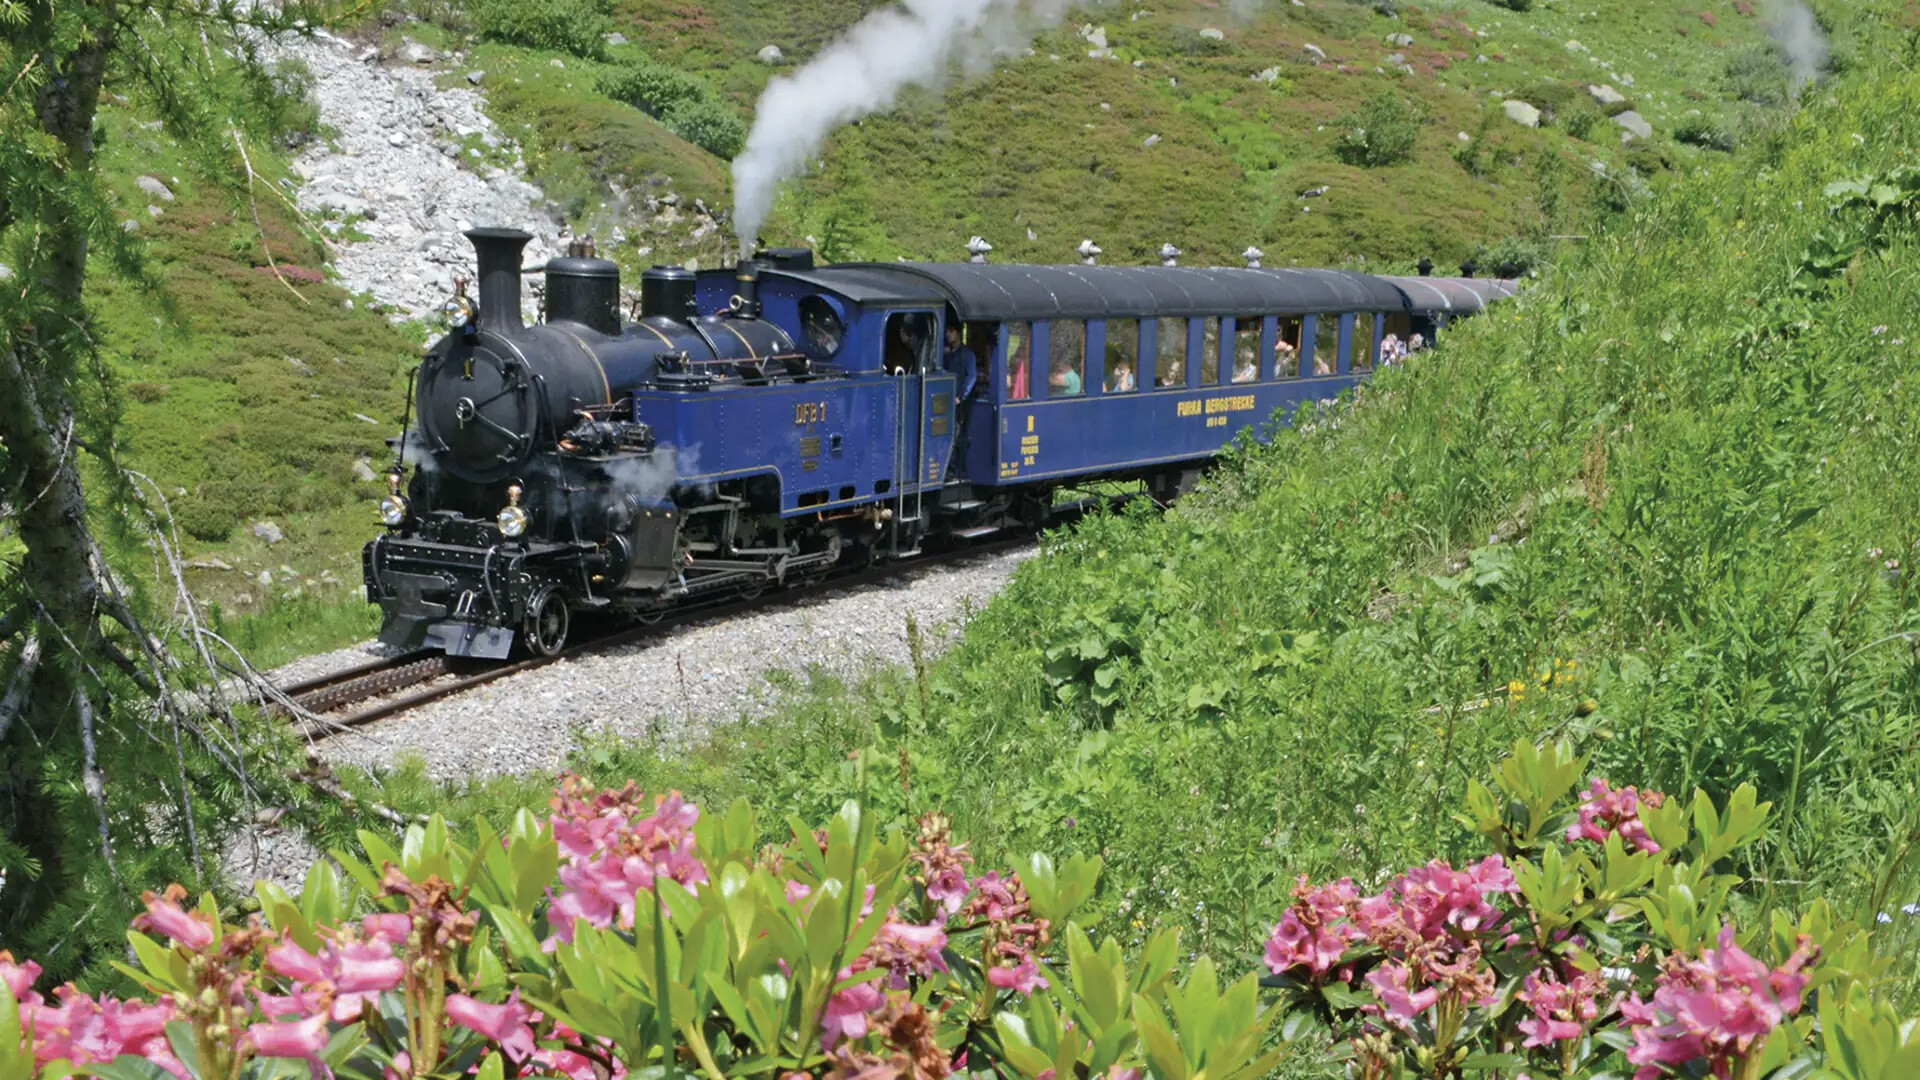
\includegraphics[width=17.5cm]{title}
	\pagebreak
	\tableofcontents
	\pagebreak
	\section{Bastian}
		\subsection{Band A}
			\subsubsection{18. Mai}
			Ich und David haben zusammen Band A geschrieben.\\
			David hat zuerst die Titelseite erstellt, ich danach die einzelnen Abschnitte.\\
			Wir haben die Aufgaben so eingeteilt das David \& ich Band A machen, da James \& Mark vieles zu tuen hatten.\\
			Ich habe die Anforderungsanalyse gemacht und ein paar Subsektionen zu unserem Vorgehensmodell hinzugefügt.\\
			Ebenfalls habe ich Aufgabe 1.5 Erledigt.
			
			\subsubsection{19. Juni}
			Ich habe zusammen mit David und James Band B angefangen.\\
			Dort habe ich auch Band B aufgabe 5 erledigt.
			
			\subsubsection{21. Juni}
			Heute habe ich vorallem 2.5 noch verbessert und das Arbeits Journal geschrieben.\\
			Wir sind jetzt kurz vor der Abgabe, vorallem fehlt uns noch das Arbeits Journal und Band D.\\
			Ich habe meinen Teil am Projekt erledigt und werde ab jetzt zur Verfügung stehen falls jemand anderes noch hilfe benötigt.
			
			
			
	\section{James}
	\section{Mark}
	\section{David}
	\subsection{Band A}
	\subsubsection{15. Mai}
	Ich habe das Github Repository erstellt. Dann habe ich den anderen erklärt, wie Latex funktioniert.\\
	Mit Mark und James musste ich noch schauen, wie man TexStudio auf Windows installiert. Das war mühsam. Am schluss haben wir es jedoch zum laufen gebracht.\\
	Wir haben auch über die Arbeitsverteilung gesprochen. Mark und James hatten während dieser Zeit viele andere Dinge geplant. Deshalb haben wir uns darauf geeinigt, dass Bastian und ich Band A schreiben werden.\\
	\subsubsection{18. Mai}
	Ich und Bastian haben zusammen Band A geschrieben. Ich habe zuerst die Titelseite für Band A geschrieben.\\
	Bastian hat dann die Abschnitte gemacht.\\
	Ich habe dann die Anforderungsanalyse gemacht. Zudem habe ich auch die Wahl des Vorgehensmodells geschrieben.\\
	Am schluss habe ich dann die Benutzereigenschaften geschrieben.
	\subsubsection{24. Mai}
	Heute ist Abgabetag. Wir haben schon alles gemacht. Mark hat es noch durchgelesen und kleine Verbesserungen vorgenommen.\\
	Ich habe nur das PDF neu generiert. Dieses habe ich dann als Release auf Github hochgeladen und dann auch abgegeben.
	\subsubsection{9. Juni}
	James hat mich gefragt, ob man in latex subsubsubsections machen kann, da er mehr Untersections brauchen könnte.\\
	Ich habe dann recherchiert und herausgefunden, wie man das macht.
	\subsubsection{14. Juni}
	Heute habe ich den Abschnitt zur Kennzeichung der Felder geschrieben. Das Bild werde ich auch noch einfügen.\\
	\subsubsection{17. Juni}
	Heute habe ich mit dem Prototypen begonnen. Da ich bei der Arbeit auch Webseiten programmiere, fällt mir das einfacher als das mit Miro oder Figma zu machen.
	\subsubsection{19. Juni}
	Als erstes habe ich die Änderungen, die ich während der Schule gemacht habe, hochgeladen. Ich habe dort am Prototyp gearbeitet.\\
	Dann habe ich im Zug an der Menu Animation gearbeitet.\\
	Zuhause habe ich dann die Kamera integration getestet. Das hat direkt funktioniert.\\
	Am Abend habe ich dann den Prototypen fertig gemacht.
	\subsubsection{21. Juni}
	Heute Abend ist der Abgabeabend. Ich habe zuerst Band B und Band C in 2 Dateien aufgeteilt, damit es weniger merge conflicts gibt.\\
	Dann habe ich github pages für den Prototypen eingerichtet. Ich hatte zuerst Probleme, die konnte ich jedoch lösen.\\
	Als ich das dann so einrichten wollte, dass es statt bei jedem Push auf den Main Branch nur bei Tags mit p* ausgelöst wird, habe ich einen Fehler erhalten. Das liegt daran, dass beim Standard nur Pages deployments vom Main Branch erlaubt werden.\\
	Als nächstes habe ich beschrieben, was ich beim Prototyp gemacht habe. Zudem habe ich noch ein paar Probleme gefunden. Diese habe ich dann verbessert.\\
	Jetzt habe ich noch den Workflow so angepasst, dass er statt npm bun verwendet. So konnte ich über 30 Sekunden Zeit sparen.\\
	Wir haben heute Gäste. Deshalb bin ich für die nächsten paar Stunden weg. Das ist mit der Gruppe so abgesprochen.
	
\end{document}